\chapter{Theory of X-ray Diffraction by Matter}\label{diffraction_theory}\noindent

This chapter gives an overview of the most important tools necessary to
understand X-ray diffraction and provides a simple framework for analysing most
CXDI experiments based on the first-order Born approximation, also known as
"kinematical" or "single-scattering" approximation. This will be of fundamental
importance when we later try to reconstruct the object that gave rise to a certain
diffraction pattern, as  it is obviously impossible to do this if we cannot
predict the diffraction pattern that a given object produces.

\section{Scattering by a free electron}\label{scat_free_electron}

According to classical electromagnetic theory the electric field associated with a plane monochromatic wave of
amplitude $E_0$, frequency $\nu$, propagating along the $z$ axis
(Fig. \ref{coordinate_axis}a), is given by
\begin{equation}
E_i(z,t) = E_0 \exp(2 \pi i \nu (t-z/c)) \, .
\label{Eq:wave_propagation}
\end{equation}
When such a wave travels through an electron of charge $e$ and mass $m$ located at the origin of a coordinate
system, that electron will oscillate in the direction of the incident electric 
vector driven by
\begin{equation}
a(t) = \frac{e E_i(0,t)}{m}
\label{Eq:electron_acceleration}
\end{equation}
with a frequency equal to the incoming wave. This in turn will make it radiate
an electric field $E_s$, like any accelerating charge. It follows from Maxwell's
equations that the electric field generated by an accelerating electron measured
at $\mathbf r$ is given by
\begin{equation}
E_s( \mathbf r,t) = \frac{e a_{\perp}(t - |\mathbf r|/c)}{4 \pi \epsilon_0 c^2 r}
\label{Eq:scattering_by_accelerating_charge}
\end{equation}
where  $\epsilon_0$ is the permittivity of free space and $a_{\perp}$ is the
acceleration projected on a plane normal to $\mathbf r$, also called the
transverse component of the acceleration (Fig. \ref{coordinate_axis}b) \cite{Attwood2007Soft}. 
\begin{figure}[h]
\centering
\includegraphics[width=1 \columnwidth]{Diffraction_Theory/coordinate_acceleration.png}
\caption{{\bf a)} Monochromatic planar wave linearly polarized along the $y$ axis
  propagating in the positive $z$ direction. {\bf b)} Transverse component of the
  acceleration sustained by the electron as observed from the position ${\mathbf r}$. $\theta$ is the angle between the polarization axis and the projection of $\mathbf r$ on a plane normal to the propagation direction.}
\label{coordinate_axis}
\end{figure}
Finally combining equations \ref{Eq:wave_propagation}, \ref{Eq:electron_acceleration} and \ref{Eq:scattering_by_accelerating_charge} we get that the instantaneous scattered field by a free electron is
\begin{eqnarray}
a_{\perp}(t) & = & |\mathbf a(t)| \sin \theta  \\
E_s(\mathbf r,t) & = & \frac{e^2 E_0 \sin \theta }{4 \pi \epsilon_0 m c^2 r}
\exp(2 \pi i \nu (t -| \mathbf r|/c)) \, . 
\label{Eq:scattering_by_electron}
\end{eqnarray}
The classical electron radius is defined as
\begin{equation}
r_e = \frac{e^2}{4 \pi \epsilon_0 m c^2}
\end{equation}
which can be used to simplify the electric field expression to
\begin{equation}
E_s(\mathbf r,t) = \frac{r_e E_0 \sin \theta }{r} \exp(2 \pi i \nu (t -| \mathbf
r|/c))  \, .
\label{Eq:scattering_by_electron_simplified}
\end{equation}
The time averaged scattered power per unit area normal to $\mathbf r$, also
known as intensity, can then be obtained from the average length of the Poynting vector,
\begin{equation} 
I(\mathbf r) = \frac{ |E_{max}(\mathbf r)|^2 }{2 \epsilon_0 c} .
\label{Eq:poynting_vector}
\end{equation}
where $E_{max}$ denotes the maximum value of the electric field.
The time averaged power per unit area normal to $\mathbf r$ scattered by an electron is then
\begin{equation}
I(\mathbf r)  = \frac{r_e^2 E_0^2 \sin^2 \theta }{2 \epsilon_0 c r^2} \, ,
\label{Eq:scattered_intensity}
\end{equation}
The total scattered intensity by a free electron as a fraction of the incoming
intensity, can now be calculated by integrating equation
\ref{Eq:scattered_intensity} over a spherical shell of radius 1 around the electron,
\begin{eqnarray}
I_0 & = & \frac{E_0^2}{2 \epsilon_0 c} \\
I_s & = & \int\limits_0^{2 \pi} \int\limits_0^{\pi} \frac{r_e^2 E_0^2 \sin^2
  \theta }{2 \epsilon_0 c} \sin \theta d \theta d\phi = \frac{8 \pi}{3}
\frac{r_e^2 E_0^2}{2 \epsilon_0 c} \\
\sigma_T & = & \frac{I_s}{I_0} = \frac{8 \pi}{3} r_e^2
\end{eqnarray}
where $I_0$ represent the incoming intensity, $I_s$ the scattered intensity and
$\sigma_T$ the ratio between the two, also known as the {\em scattering cross-section}
for a free electron, also known as the Thomson cross-section after the British
physicist J.J. Thomson who first derived it in the beginning of the 20th
century. Elastic scattering by a free charged particle is also known as {\em Thomson scattering}.

\section{Scattering by two electrons}\label{scat_two_electrons}

If instead of just one electron we have a system composed of two or more
electrons a new phenomenon is observed, {\em interference} between the waves
scattered by the different electrons. We will start by looking at the most simple
system where this occurs, one with just two electrons. We will keep the electron
from the previous section at the origin and add a new electron at the position
$\mathbf r$. When the system is illuminated by an electric field of amplitude $E_0$
traveling along $\mathbf s_0$, both electrons will scatter as described in
Eq. \ref{Eq:scattering_by_electron_simplified}. The amplitude of the scattered
field from each electron is the same but the phase depends on the relative position of
the two electrons (Fig. \ref{Fig:two_electrons}). 

\begin{figure}[h]
\begin{center}
\includegraphics[width=0.7 \columnwidth]{Diffraction_Theory/two_electrons.png}
\end{center}
\caption{Monochromatic planar wave propagating along $\mathbf s_0$, shines on two
  electrons separated by $\mathbf r$. The observed scattered electric field on the
  direction $\mathbf s$ at a distance $| \mathbf d|$ much larger than $|\mathbf r|$ is the
  sum of two identical fields separated by a phase difference dependent on the
  path difference $\Delta l_1 + \Delta l_2$ \cite{2001International}.}
\label{Fig:two_electrons}
\end{figure}
For an observer located at $\mathbf d$ in the direction of $\mathbf s$, at a distance
much greater than the distance between the electrons the observed total electric
field is the sum of the fields scattered by each of the electrons, which can be
approximated by,
\begin{eqnarray}
\Delta l & = & \Delta l_1 + \Delta l_2 = \mathbf r \cdot (\mathbf s_0 - \mathbf s)\\
E(\mathbf d) & = & E_s(\mathbf d) + E_s(\mathbf d) \exp(\frac{2 \pi i \Delta
  l}{\lambda})
\label{Eq:ScatteringTwoElectrons}
\end{eqnarray}
where $\mathbf s_0$ and $\mathbf s$ are unit vectors, $\Delta l$ is the total path
difference, $E_s$ the electric field scattered by an isolated electron, $\lambda$
the wavelength of the incoming field and $E$ the total observed field.
This approximation assumes that $|\mathbf d| -
|\mathbf d- \mathbf a| << \lambda$, or put in another way $|\mathbf r|^2/(|\mathbf d| \lambda) \ll
1 $. This approximation is known as the {\em Fraunhofer approximation} and the conditions
under which they are valid are known as the far field regime. ``Fraunhofer
diffraction'' is a term used to describe diffraction in this regime. Also implicit
in this calculation is the assumption that the scattered field from one electron produces a
negligible influence on the scattered field of the other electron, that is, multiple
scattering can be ignored. This approximation is known as the {\em first-order Born
  approximation}.
It is
important to notice that the relative phase between the two electrons does not
depend on the choice of origin and so the observed intensity is independent of
the choice of origin, as it must obviously be. 


\section{Scattering by an arbitrary electron cloud}\label{scat_cloud}

The two electron framework presented in the previous section can be easily
extended to $N$ electrons by noticing that the electrons scatter independently
of each other. So the scattering of $N$ electrons measured at a point $\mathbf d$
is given by
\begin{equation}
E(\mathbf d) = E_s(\mathbf d) \sum_{n=0}^N \exp\left(\frac{2 \pi i \mathbf r_n \cdot(\mathbf s_0 -
\mathbf s)}{\lambda}\right) \, .
\end{equation}
The vector $\mathbf S = \frac{\mathbf s_0 - \mathbf s}{\lambda}$ is known in crystallography
as the {\em scattering vector} and the surface drawn by the tip of the
scattering vector while $\mathbf s$ is rotated around a sphere is known as the
{\em Ewald sphere}.

The continuous case is now easily derived by replacing individual electrons by
an electron density $\rho$. The scattering from an electron density cloud is
then described by
\begin{equation}
E(\mathbf d) = E_s(\mathbf d) \int_{\mathbf r} \rho(\mathbf r) \exp\left(2
    \pi i \mathbf r \cdot \mathbf S \right) d\mathbf r\, .
\end{equation}
We can now introduce the {\em structure factor}, defined as the ratio between
the scattered field by the system and the scattered field by a single
electron,
\begin{equation}
F(\mathbf d) = \frac{E(\mathbf d)}{E_s(\mathbf d)} = F\left(\frac{\mathbf d}{|\mathbf d|}\right)
\end{equation}
The structure factor is a more useful quantity than the electric field as it does not depend
on the distance to the detector, only on the direction of the observer and the
structure of the system. For an arbitrary electron cloud the structure factor as
a function of the scattering vector is given by,
\begin{equation}
F(\mathbf S) = \int_{\mathbf r} \rho(\mathbf r) \exp\left(2
    \pi i \mathbf r \cdot \mathbf S \right) d\mathbf r\, ,
\end{equation}
which is simply the three dimensional Fourier transform of $\rho(\mathbf r)$
evaluated at $\mathbf S$. It is for this reason that Fourier transforms are such
a useful tool when studying diffraction, and why they were introduced in the
previous chapter.

This formalism was used for the diffraction calculation in {\bf paper \ref{melting}}.

\section{Coherence}\label{coherence}

Throughout the previous sections we have assumed that the incoming wave was
perfectly coherent, both temporaly and spatially (see Fig. \ref{Fig:coherence}). Temporal coherence is related
to the bandwidth of the wave: the larger the bandwidth the worse is the
coherence. We have assumed monochromatic waves i.e. perfect temporal
coherence. Spatial coherence is a measure of how stable is the phase relation between
two points as a function of time. More accurately it is the cross-correlation of the field at two locations over time \cite{Attwood2007Soft}. 

Coherence is important for diffraction experiments \cite{HauRiege2008Effect,Whitehead2009Diffractive} because if, for example, the
spatial coherence of the beam is low, the instantaneous diffraction pattern of
our system will change rapidly during the exposure, but the integrated pattern
will show very few signs of interference between different parts of the
system and so hide its structure. We can see this by comparing the diffraction
pattern obtrain from the field in Eq. \ref{Eq:ScatteringTwoElectrons}, to the
one generated by replacing $\Delta l/\lambda$ by a random term $X$
between $-1/2$ and $1/2$ corresponding to a random phase difference due to
spatial incoherence. In the coherent case we get:
\begin{eqnarray}
  I(\mathbf d)  & \propto & |E_s(\mathbf d) + E_s(\mathbf d) \exp(\frac{2 \pi i \Delta
    l}{\lambda})|^2  = \nonumber \\
 & = & 2 |E_s(\mathbf d)|^2 + 2 |E_s(\mathbf d)|^2
  \cos(2 \pi \Delta l / \lambda)
\end{eqnarray}
 while in the incoherent case we have
\begin{eqnarray}
 E(\mathbf d,X) & = &  E_s(\mathbf d) + E_s(\mathbf d) \exp(2 \pi i X) \nonumber
 \\
I(\mathbf d)  & \propto & \int_{-1/2}^{1/2} |E(\mathbf d,X)|^2 dX = 2 |E_s(\mathbf d)|^2
\end{eqnarray}
where $I(\mathbf d)$ is the observed diffracted intensity. Notice that in the
incoherent case the term $2 |E_s(\mathbf d)|^2 \cos(2 \pi \Delta l / \lambda)$,
which gives information about the relative location of the two electrons, is not
present. This term is usually called the cross term and is the only one that
gives structural information. The other term is called the self term, and this only gives
information about the building blocks of the system, the electrons in this case,
but not how they are organized.

\begin{figure}[h]
\begin{center}
\includegraphics[width=1.0 \columnwidth]{Diffraction_Theory/coherence.pdf}
\end{center}
\caption{{\bf Coherence.} A light bulb is a source of incoherent radiation, but by passing it
  through a pinhole it is possible to make it spatially coherent and by
  filtering it down to a single wavelength it is possible to make it temporally coherent. 
}
\label{Fig:coherence}
\end{figure}

Motion in the system during the exposure can also produce effects similar to
the ones produced by an incoherent wave, if the motion is of the order of the probing
wavelength. In a way, one can say that the stability of the sample also affects
the coherence of the diffraction experiment. This effect is analysed in detail
in {\bf paper \ref{dynamics}}.

%%% Local Variables: 
%%% mode: latex
%%% TeX-master: "../Thesis"
%%% End: 
